\section{Hardware and setup}

\subsection{Raytrix Technology}\label{the_raytrix_camera}

\begin{figure}[ht]
    \centering
    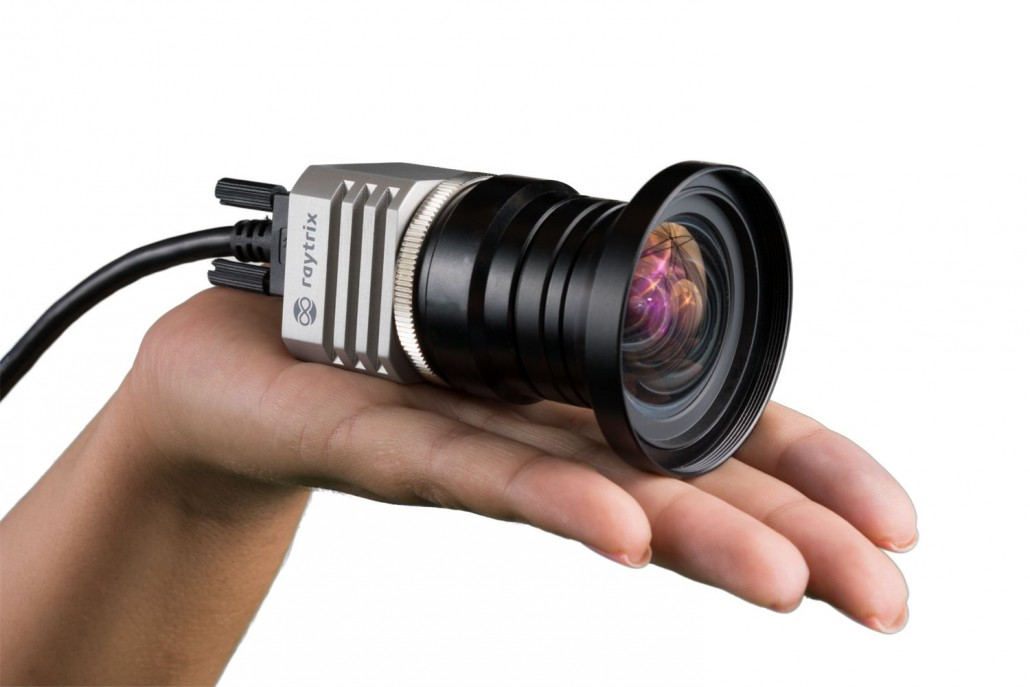
\includegraphics[width=.9\linewidth]{images/introduction/raytrix_camera}
    \caption{Raytrix R42 Camera}
    \label{fig:raytrix_camera}
\end{figure}

The camera used throughout this project is the Raytrix R42 camera. The camera is developed by Raytrix, a German company which offers several 3D Light Field cameras intended for professional and industrial use. The R42 is their highest resolving light field camera to date. It is based on a 42 megaray sensor and offers an effective resolution up to 10 megapixels at 7 FPS. \cite{website:raytrix_r42}

Light Field cameras are a new type of 3D-cameras that capture a standard image together with the depth information of a scene. Metric 3D information can be captured with a single light field camera through a single lens in a single shot using just the available light. Raytrix has specialized on developing light field cameras for industrial applications. A patented micro lens array design allows for an optimal compromise between high effective resolution and large depth of field. Raytrix cameras are already in use in applications like volumetric velocimetry, plant phenotyping, automated optical inspection and microscopy, to name a few. \cite{website:raytrix_main}

This camera is therefore very useful for industrial purposes, as you can get both a clear image, a depth map, and a 3D model of the scene. It has though no documented use underwater, and since the physical properties of water cause degradation effects not present in air, the depth measurements get affected. We get both "holes" in the object, and detected particles in front of the object. If we are going to use this camera technology to measure volume of objects underwater, we need to improve the data received from the camera. Particles in front needs to be removed, and holes need to be filled with appropriate data. Setting the right light is also something that must be tested. 

The Raytrix camera is build up by a main lens in front, a micro lens array, and the image sensor behind. The micro lens array has many thousand micro lenses, 2600x4000 lenses. The micro lens array is placed in front of the image sensor inside the camera, which turns the image sensor into a micro-camera array (see figure \ref{fig:light_field}), where each micro-camera sees part of the intermediate image from a slightly different perspective. That is, instead of using a large camera array that looks at the object directly, we can choose a main lens to select the desired field-of-view and create the intermediate image in front of the micro camera array. The images generated by the camera in this setup are processed on a PC with appropriate software algorithms to calculate the scene depth and to reconstruct a 2D image. When all processing is done on a GPU, it allows for high resolution 2D and 3D images, at up to 7 FPS. \cite{website:raytrix_technology}

\begin{figure}[h]
    \centering
    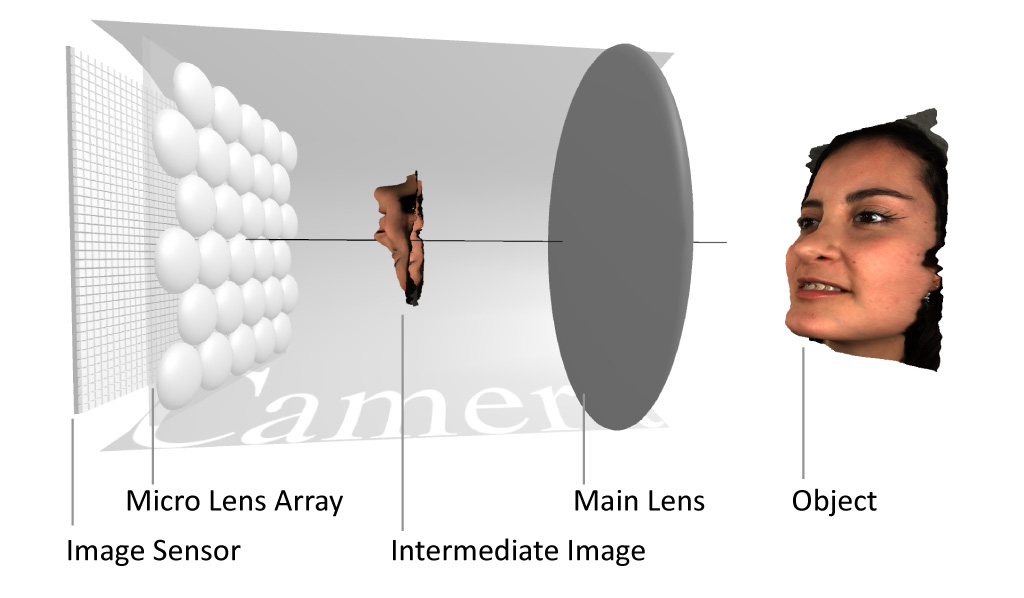
\includegraphics[width=.9\linewidth]{images/introduction/Light-Field-Camera-Schematic}
    \caption{Raytrix Light Field Technology}
    \label{fig:light_field}
\end{figure}

When calibrating the camera the raw image is used to make sure the main objects edges are shown in several of the micro lenses. The more micro lenses picking up one object, the more accurate the depth measurement. 

The raw image shows the capture from all micro lenses, as seen in figure \ref{fig:raw_image}. The camera perform no processing internally, it simply deliver a raw image to a PC, which is then processed on a GPU to obtain the 2D and 3D data. 
The totalfocus image - which is just a normal color image - is made from the raw image on a computer, figure \ref{fig:totalfocus}. 
The depthmap, figure \ref{fig:depthmap}, is computed from the raw image, and the 3D image, figure \ref{fig:3d_image}, is made from the depthmap and the totalfocus image. 
The depth in the depthmap is represented by colors, where red is close to the camera, yellow and green is the object centered during calibration, blue is behind the object, and black has no depth. This means that the optimal depthmap image would be all black, with a yellow and green fish.

\begin{figure}[h]
    \centering
    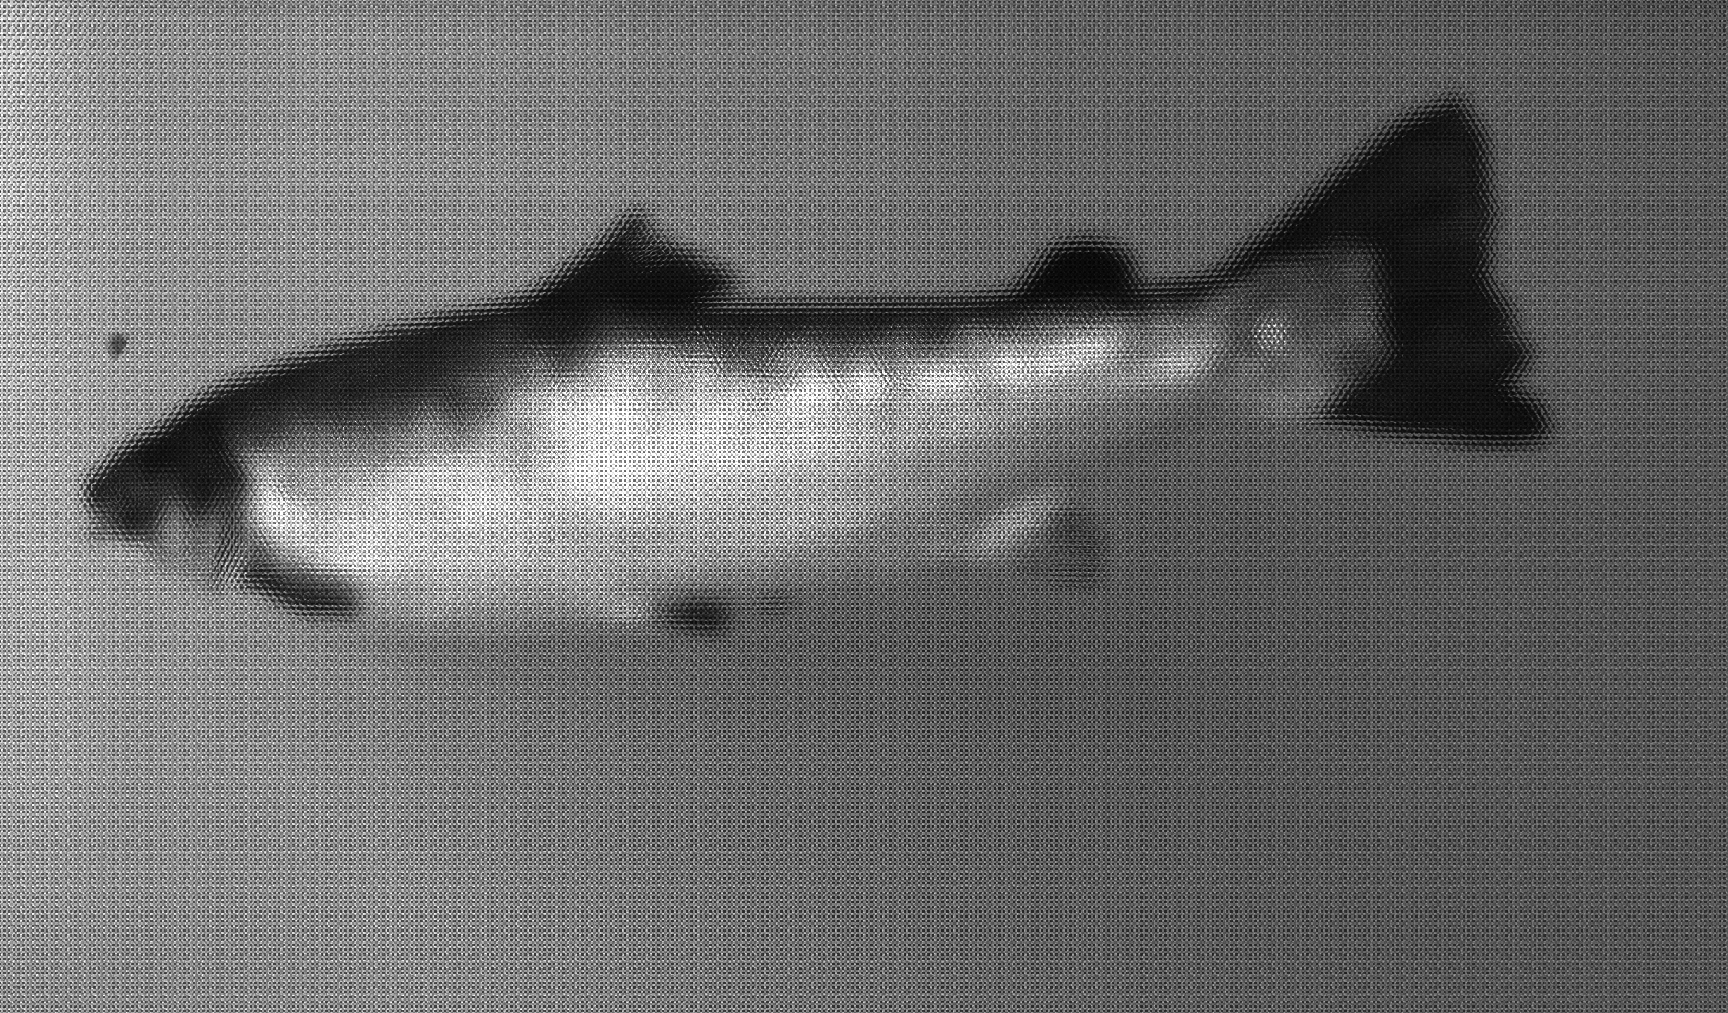
\includegraphics[width=.9\linewidth]{images/introduction/raw}
    \caption{Raw image}
    \label{fig:raw_image}
\end{figure}

\begin{figure}[h]
    \centering
    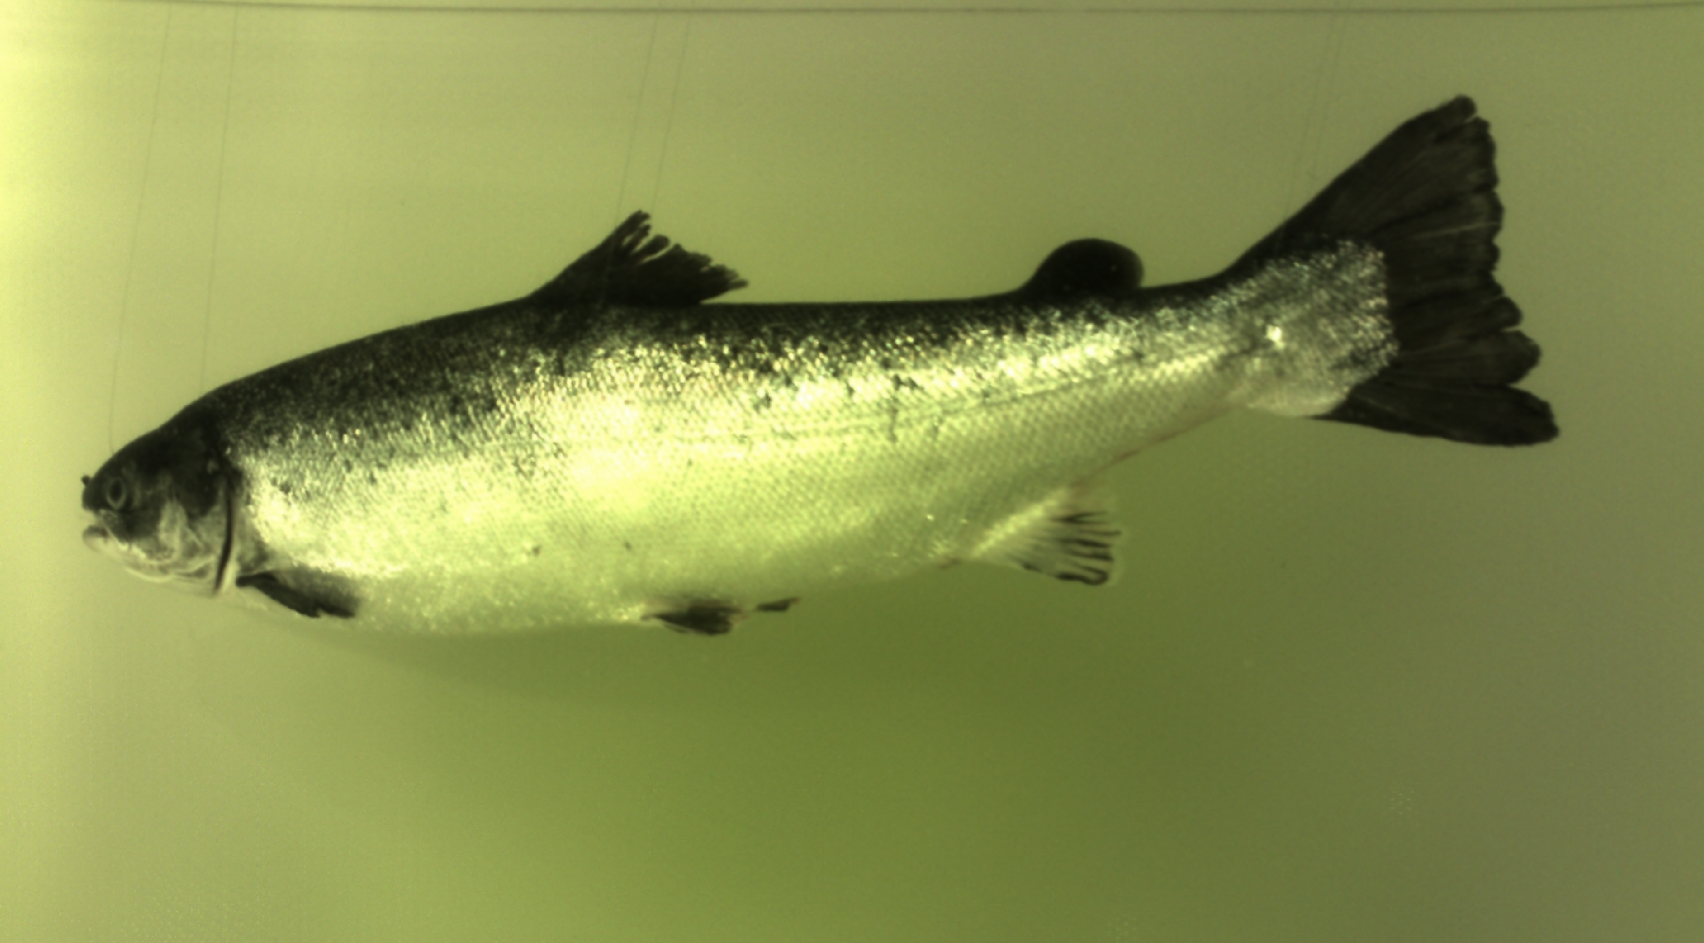
\includegraphics[width=.9\linewidth]{images/introduction/totalfocus}
    \caption{Totalfocus image}
    \label{fig:totalfocus}
\end{figure}

\begin{figure}[h]
    \centering
    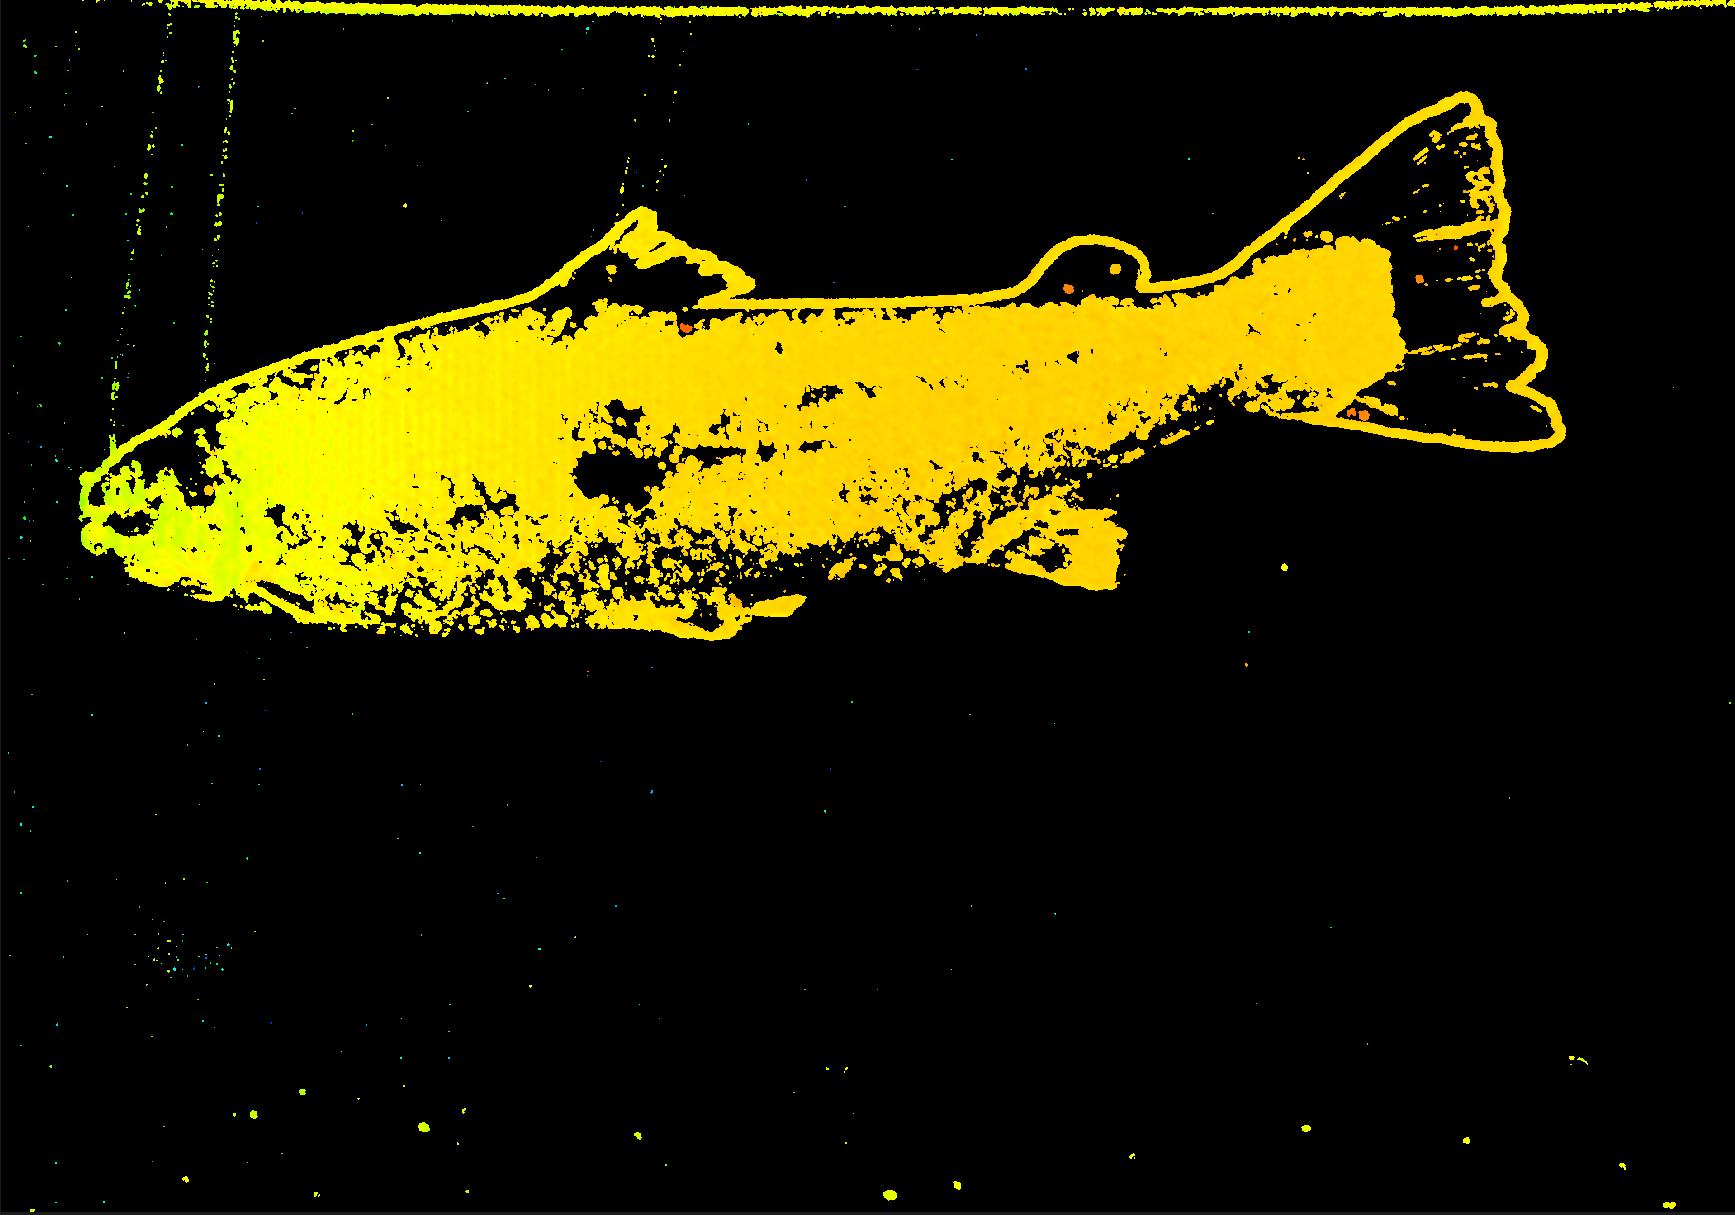
\includegraphics[width=.9\linewidth]{images/introduction/depthmap}
    \caption{Depthmap image}
    \label{fig:depthmap}
\end{figure}

\begin{figure}[h]
    \centering
    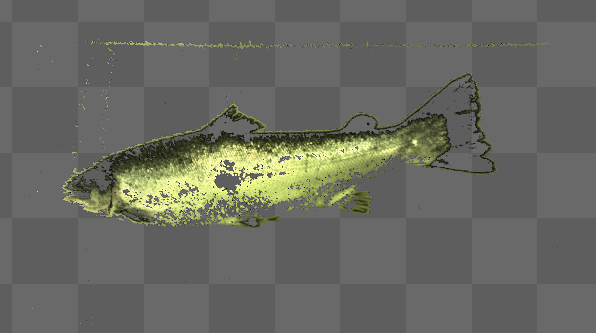
\includegraphics[width=.9\linewidth]{images/introduction/depth3D}
    \caption{3D image}
    \label{fig:3d_image}
\end{figure}

As seen from the 3D image produced in the Raytrix Software, the particles in front will affect the surface of the object. The same goes for holes in the object. Figure \ref{fig:3d_image_side} shows the 3D image in figure \ref{fig:3d_image} turned about 45 degrees to the side. This shows how inaccurate the current 3D model for underwater images are. 

\begin{figure}[h]
    \centering
    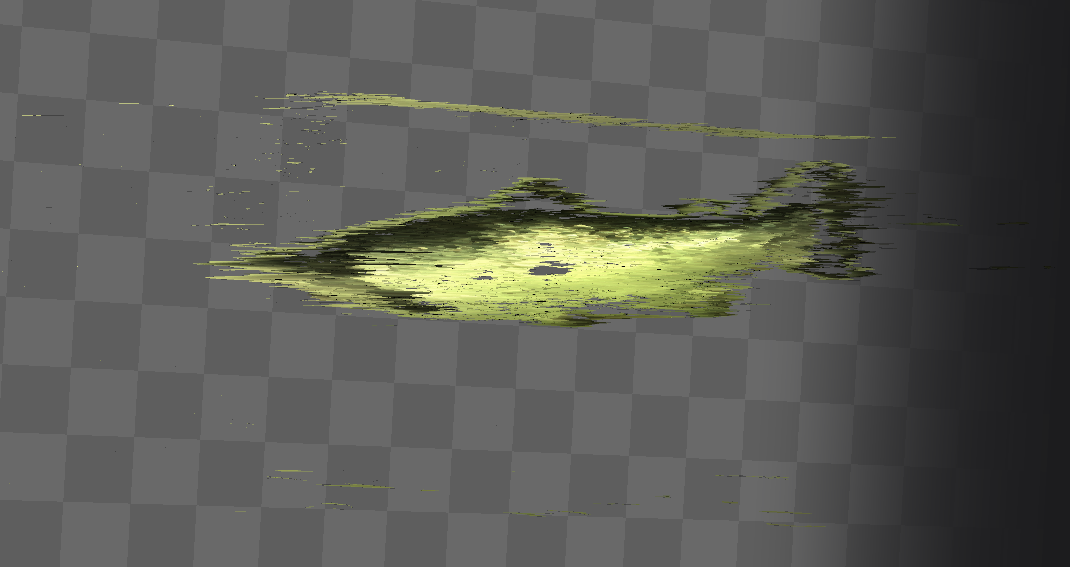
\includegraphics[width=.9\linewidth]{images/introduction/depth3D_side}
    \caption{3D image from the side}
    \label{fig:3d_image_side}
\end{figure}

The reason the Raytrix R42 camera is used by Sensomar SEALAB, is because of its high resolution and high frame-rate. All competitors of Raytrix does not have as good frame-rate and resolution all together. The Raytrix camera is also different from other light field cameras because it has the light ray crossing behind the micro lens array, while other light field cameras have the light crossing in front of the micro lens array.

One problem working with the Raytrix is that the depth information is stored in their own .ray format. It is not yet possible to do direct image processing on this format using other processing tools than Raytrixs own software, RxLive. RxLive has some good software tools, but to do more advanced image processing the software is not sufficient.
Another problem is the calibration of the Raytrix. For every time the camera is calibrated the colors in the depthmap, representing the depth, change. ....

All images in this subsection is made with the Raytrix software, RxLive 4.0.



{\color{red}Explain more about how the Raytrix measures depth?? Explain the calibration and the RAW image?? And about Light Field Cameras?}



%%%%%%%%%%%%%%%%%%%%%%%%%%%%%%%%%%%%%%%%%%%%%%%%%%%%%%%%%%%%%%%%%%%%%%


\subsection{Wetlab}\label{wetlab}

SEALAB has its own test facilities where they have the complete camera setup in a small pool. Aquaculture companies deliver fish for testing.


